\documentclass[a4paper,11pt]{article}
\usepackage[verbose,a4paper,tmargin=2cm,bmargin=2cm,lmargin=2.5cm,rmargin=2.5cm]{geometry}
\usepackage[utf8]{inputenc}
\usepackage{polski}
\usepackage{amsmath}
\usepackage{amsfonts}
\usepackage{amssymb}
\usepackage{lastpage}
\usepackage{indentfirst}
\usepackage{verbatim}
\usepackage{graphicx}
\usepackage{fancyhdr}
\usepackage{listings}
\usepackage{float}
\usepackage{hyperref}
\hypersetup{
    colorlinks = true,
    linkcolor = black,
    urlcolor = cyan
}
\usepackage{xcolor}
\usepackage{tikz}
\usepackage{multirow}
\frenchspacing
\pagestyle{fancyplain}
\fancyhf{}

\usepackage{setspace}

\renewcommand{\headrulewidth}{0pt}
\renewcommand{\footrulewidth}{0.4pt}
\newcommand{\degree}{\ensuremath{^{\circ}}} 
\fancyfoot[L]{MUM: P. Galewicz, B. Jurczewski, Z. Nowacki, K.Podlewski, P. Wardęcki}
\fancyfoot[R]{\thepage\ / \pageref{LastPage}}

\begin{document}

\begin{titlepage}
\begin{center}
\begin{tabular}{rcl}
\begin{tabular}{|r|}
\hline \\
\large{\underline{234053~~~~~~~~~~~~~~~~~~~~~~~} }\\
\small{\textit{Numer indeksu}}\\
\large{\underline{Paweł Galewicz~~~~~~~~~~~~} }\\
\small{\textit{Imię i nazwisko}}\\\\ \hline
\end{tabular} 
&
\begin{tabular}{|r|}
\hline \\
\large{\underline{234067~~~~~~~~~~~~~~~~~~~~~~~} }\\
\small{\textit{Numer indeksu}}\\
\large{\underline{Bartosz Jurczewski~~~~~~~} }\\
\small{\textit{Imię i nazwisko}}\\\\ \hline
\end{tabular} 
&
\begin{tabular}{|r|}
\hline \\
\large{\underline{234102~~~~~~~~~~~~~~~~~~~~~~~} }\\
\small{\textit{Numer indeksu}}\\
\large{\underline{Zbigniew Nowacki~~~~~~~~} }\\
\small{\textit{Imię i nazwisko}}\\\\ \hline
\end{tabular} 
\end{tabular} 

        \vspace{10px}

\begin{tabular}{rl}
\begin{tabular}{|r|}
\hline \\
\large{\underline{234106~~~~~~~~~~~~~~~~~~~~~~~} }\\
\small{\textit{Numer indeksu}}\\
\large{\underline{Karol Podlewski~~~~~~~~~~~} }\\
\small{\textit{Imię i nazwisko}}\\\\ \hline
\end{tabular} 
&
\begin{tabular}{|r|}
\hline \\
\large{\underline{234128~~~~~~~~~~~~~~~~~~~~~~~} }\\
\small{\textit{Numer indeksu}}\\
\large{\underline{Piotr Wardęcki~~~~~~~~~~~~} }\\
\small{\textit{Imię i nazwisko}}\\\\ \hline
\end{tabular} 
\end{tabular}
\end{center}

\vspace{25px}

\begin{tabular}{ll}
\LARGE{\textbf{Kierunek}}& \LARGE{Informatyka Stosowana} \\
\LARGE{\textbf{Stopień}}& \LARGE{II} \\
\LARGE{\textbf{Specjalizacja}}& \LARGE{Data Science} \\
\LARGE{\textbf{Semestr}}& \LARGE{1} \\\\
\LARGE{\textbf{Data oddania}}& \LARGE{18 marca 2020} \\\\\\\\\\\\\\
\end{tabular}

\begin{center}
\textbf{\huge{\\~\\Metody uczenia maszynowego }}
\textbf{\Huge{\\~\\Problem set 1}}
\end{center}

\end{titlepage}

\setcounter{page}{2}
\setstretch{1.5}
\tableofcontents
\newpage
\setstretch{1.1}

\section{Cel} \label{sec:cel}
Zadanie polegało na analizie procesu klasyfikacji danych za pomocą wybranych metod:

\begin{enumerate}
    \item Algorytm drzew decyzyjnych
    \item Naiwny klasyfikator Bayesa
    \item Maszyna wektorów nośnych
    \item Klasyfikator k-najbliższych sąsiadów
    \item Algorytm sztucznych sieci neuronowych
\end{enumerate}

Należało zaimplementować każdą metodę, a następnie zweryfikować jej działanie biorąc pod uwagę:

\begin{itemize}
    \item rożne możliwe ustawienia parametrów konfiguracyjnych i ich wpływ na wyniki klasyfikacji
    \item zbiory danych o różnej charakterystyce (przynajmniej 3 różne zbiory)
\end{itemize}

Każdą metodę należało przetestować na tych samych zbiorach, a następnie porównać wyniki i wyciągnąć wnioski dotyczące skuteczności poszczególnych metod. Jako kryterium porównawcze wykorzystaliśmy dokładność klasyfikacji.

\section{Opis implementacji}
Algorytmy zostały zaimplementowane za pomocą języka Python w wersji 3.8.2.
Wykorzystano w nim biblioteki NumPy, Sklearn i Pandas. Bazowaliśmy na trzech zestawach danych: 
\begin{itemize}
    \item{\href{https://www.kaggle.com/pitasr/falldata}{Fall Detection Data from China}}
    \item{\href{https://www.kaggle.com/jsphyg/weather-dataset-rattle-package}{Rain in Australia}}
    \item{\href{https://www.kaggle.com/russellyates88/suicide-rates-overview-1985-to-2016}{Suicide Rates Overview 1985 to 2016}}
\end{itemize}

\section{Klasyfikatory}

\subsection{Algorytm drzew decyzyjnych}
Algorytm polega na stworzeniu modelu do przewidywania wartości na podstawie prostych reguł wywnioskowanych z danych treningowych. Reguły te tworzone są w struktury drzewiaste. Struktury te składają się z:

\begin{itemize}
    \item węzła głównego -- od niego rozpoczyna się proces decyzyjny
    \item węzłów decyzyjnych -- zawierające reguły-zapytania
    \item stanów (liścia) -- końcowych stanów algorytmu, w problemie klasyfikacji są one równoważne z etykietami
    \item połączeń między węzłami -- reprezentującymi możliwe warianty dla danego
\end{itemize}

Zapytania w węzłach są wyrażeniami logicznymi dotyczącymi jednej z cech modelu oraz jej wartości. Wartość ta dobrana musi być w taki sposób, żeby jak najlepiej wydzielić klasę obiektów z przychodzących na węźle danych. Można wtedy powiedzieć, że dany węzeł dostarcza najwięcej informacji. Na potrzebę obliczenia tego przyrostu informacji wprowadza się kryterium \textit{Ipurity}, którego sensem jest fakt, czy po podziale w danym węźle dane zostały poprawnie klasyfikowane. Dokładny sposób wyliczania wartości tego kryterium jest zależny od konfiguracji.
\par
Drzewa domyślnie budowane są do momentu zminimalizowania wartości Impurity, przez co struktura drzew może być bardzo złożona. Skutkiem tego może być przeuczenie modelu, co rzutuje na jego dokładność. Aby ograniczyć możliwość wystąpienia tego zjawiska wprowadza się dodatkowy parametr --  \textit{maksymalna głębokość} -- który mówi o tym ile najwięcej rozgałęzień może wystąpić między węzłem głównym a liściem.

\subsection{Naiwny klasyfikator Bayesa}
Naiwny klasyfikator Bayesa dokonuje klasyfikacji na bazie twierdzenia Bayesa:
$$ P(A \mid B) = \frac{P(B \mid A) \, P(A)}{P(B)} $$
gdzie:
\begin{itemize}
    \item $A$, $B$ -- zdarzenia
    \item $P(A \mid B)$ -- prawdopodobieństwo zdarzenia $A$, o ile zajdzie $B$
    \item $P(B \mid A)$ -- prawdopodobieństwo zdarzenia $B$, o ile zajdzie $A$
    \item $P(A)$ -- prawdopodobieństwo wystąpienia zdarzenia $A$
    \item $P(B)$ -- suma prawdopodobieństw wszystkich potencjalnych skutków zdarzenia: $P(B)=\sum P(B\mid A)P(B)$
\end{itemize}

Model naiwnego klasyfikatora Bayesa zakłada, że dana cecha klasy jest niepowiązana z pozostałymi cechami. Każda z cech indywidualnie wskazuje na prawdopodobieństwo przynależności do danej klasy.
Sprawdza się najlepiej przy dużych zbiorach danych. Jest wykorzystywany m.in. przy filtrowaniu spamu, diagnozie medycznej, czy prognozowaniu pogody.

\subsection{Maszyna wektorów nośnych}
Maszyna wektorów nośnych jest klasyfikatorem liniowym. Algorytm polega na rozdzieleniu obiektów o różnej przynależności klasowej za pomocą hiperpłaszczyzn, które mają być od siebie możliwe jak najbardziej oddalone - taką odległość nazywa się marginesem klasyfikatora, a hiperpłaszczyzny z największym marginesem wektorami nośnymi. 

Algorytm bardzo dobrze sobie radzi z danymi liniowo separowanymi, ale nie zawsze będzie istniała hiperpłaszczyzna rozdzielająca, która zapewni poprawną klasyfikację wszystkich elementów zbioru. W takich przypadkach maszyna wektorów nośnych za pomocą funkcji jądrowych transformuje przestrzeń do postaci liniowo separowanej.

\subsection{Klasyfikator k-najbliższych sąsiadów}
Algorytm k najbliższych sąsiadów jest klasyfikatorem (ściślej algorytmem regresji regresji nieparametrycznej). Algorytm ten zakłada dany zbiór uczący, w którym znajdują się już sklasyfikowane dane. Schemat składa się z szukania \textit{k} obiektów najbliższych do obiektu klasyfikowanego. Następnie, przyporządkowuje się nowy obiekt do najczęściej występującej klasy w obrębie jego k-najbliższych sąsiadów.\\

Rysunek \ref{fig:knn} pokazuje działanie algorytmu. W przypadku k=3 (mniejszy okrąg), różowa kropka zostanie zakwalifikowana do niebieskich trójkątów. W przypadku k=5 (większy okrąg) - do pomarańczowych kwadratów.

\begin{figure}[!htbp]
    	\centering
    	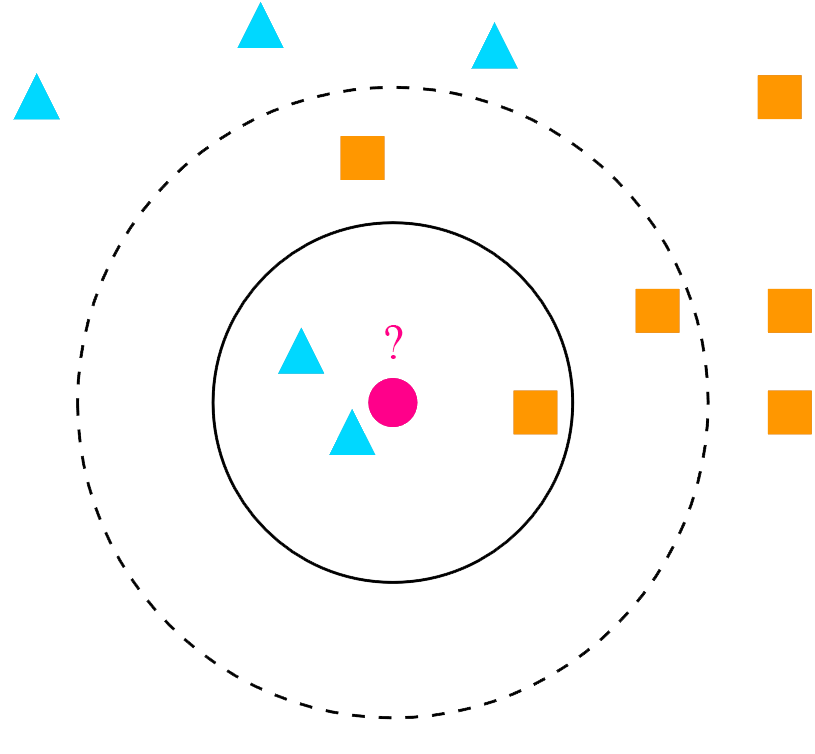
\includegraphics[width=0.45\textwidth]{images/knn.png}
    	\caption{ Wizualizacja klasyfikatora k-najbliższych sąsiadów}
    	\label{fig:knn}
\end{figure}

\subsection{Algorytm sztucznych sieci neuronowych}
Sztuczna siec neuronowa  jest połączeniem wielu elementow nazywanych sztucznymi neuronami, które tworzą conajmniej trzy warstwy: wejściową, ukrytą oraz wyjściową. Neurony przetwarzają informacje dzięki nadaniu im parametrów które nazywane są wagami. Podstawą tworzenia sieci neuronowej jest modyfikowanie współczynnika wagowego połączeń w celu uzyskania poprawnych wyników.

\section{Badania}
W tabelach \ref{tab:dataset1}, \ref{tab:dataset2}, \ref{tab:dataset3} zaprezentowano porównanie dokładności algorytmów dla różnego procentowego podziału datasetu na dane treningowe i testowe. Numeracja algorytmów na podstawie punktu \ref{sec:cel} sprawozdania.

\subsection{Fall Detection Data from China}
\begin{table}[H]
\centering
\begin{tabular}{|l|l|l|l|l|l|}
\hline
\multicolumn{1}{|c|}{\multirow{2}{*}{\textbf{Procent danych treningowych}}} & \multicolumn{5}{c|}{\textbf{Numer algorytmu}}                       \\ \cline{2-6}
\multicolumn{1}{|c|}{}                                                      & \textbf{1} & \textbf{2} & \textbf{3} & \textbf{4} & \textbf{5} \\ \hline
10\%                                                                        & 0.559       & 0.161       & 0.296       & 0.551       & 0.29        \\ \hline
20\%                                                                        & 0.618       & 0.159       & 0.306       & 0.598       & 0.392       \\ \hline
30\%                                                                        & 0.619       & 0.18        & 0.302       & 0.61        & 0.302       \\ \hline
40\%                                                                        & 0.647       & 0.136       & 0.318       & 0.626       & 0.393       \\ \hline
50\%                                                                        & 0.657       & 0.135       & 0.299       & 0.644       & 0.387       \\ \hline
60\%                                                                        & 0.668       & 0.132       & 0.298       & 0.65        & 0.307       \\ \hline
70\%                                                                        & 0.695       & 0.139       & 0.306       & 0.65        & 0.391       \\ \hline
80\%                                                                        & 0.687       & 0.155       & 0.319       & 0.661       & 0.332       \\ \hline
90\%                                                                        & 0.692       & 0.146       & 0.329       & 0.668       & 0.348       \\ \hline
\end{tabular}
\caption{Porównanie dokładności algorytmu dla datasetu 1}
\label{tab:dataset1}
\end{table}

\subsection{Rain in Australia}

\begin{table}[H]
\centering
\begin{tabular}{|l|l|l|l|l|l|}
\hline
\multicolumn{1}{|c|}{\multirow{2}{*}{\textbf{Procent danych treningowych}}} & \multicolumn{5}{c|}{\textbf{Numer algorytmu}}                       \\ \cline{2-6}
\multicolumn{1}{|c|}{}                                                      & \textbf{1} & \textbf{2} & \textbf{3} & \textbf{4} & \textbf{5} \\ \hline
10\%                                                          & 1.0         & 0.938       & 0.78        & 0.839       & 0.976       \\ \hline
20\%                                                        & 1.0         & 0.938       & 0.783       & 0.846       & 0.978       \\ \hline
30\%                                                         & 1.0         & 0.944       & 0.784       & 0.848       & 0.967       \\ \hline
40\%                                                          & 1.0         & 0.941       & 0.789       & 0.857       & 0.98        \\ \hline
50\%                                                         & 1.0         & 0.943       & 0.8         & 0.86        & 0.981       \\ \hline
60\%                                                          & 1.0         & 0.943       & 0.807       & 0.86        & 0.994       \\ \hline
70\%                                                          & 1.0         & 0.945       & 0.81        & 0.866       & 0.977       \\ \hline
80\%                                                          & 1.0         & 0.943       & 0.82        & 0.862       & 0.995       \\ \hline
90\%                                                          & 1.0         & 0.942       & 0.816       & 0.857       & 0.991       \\ \hline
\end{tabular}
\caption{Porównanie dokładności algorytmu dla datasetu 2}
\label{tab:dataset2}
\end{table}

\subsection{Suicide Rates Overview 1985 to 2016} 

\begin{table}[H]
\centering
\begin{tabular}{|l|c|c|c|c|c|}
\hline
\multicolumn{1}{|c|}{\multirow{2}{*}{\textbf{Procent danych treningowych}}} & \multicolumn{5}{c|}{\textbf{Numer algorytmu}}                       \\ \cline{2-6}
\multicolumn{1}{|c|}{}                                                      & \textbf{1} & \textbf{2} & \textbf{3} & \textbf{4} & \textbf{5} \\ \hline
10\%                                                                   & 0.211      & 0.172      & 0.109      & 0.227      & 0.36       \\ \hline
20\%                                                                   & 0.254      & 0.202      & 0.137      & 0.246      & 0.367      \\ \hline
30\%                                                                   & 0.22       & 0.175      & 0.211      & 0.215      & 0.328      \\ \hline
40\%                                                                   & 0.231      & 0.183      & 0.183      & 0.22       & 0.403      \\ \hline
50\%                                                                   & 0.224      & 0.228      & 0.244      & 0.195      & 0.456      \\ \hline
60\%                                                                   & 0.215      & 0.187      & 0.264      & 0.212      & 0.538      \\ \hline
70\%                                                                   & 0.221      & 0.262      & 0.254      & 0.208      & 0.331      \\ \hline
80\%                                                                   & 0.198      & 0.229      & 0.302      & 0.219      & 0.538      \\ \hline
90\%                                                                   & 0.25       & 0.213      & 0.088      & 0.229      & 0.36       \\ \hline
\end{tabular}
\caption{Porównanie dokładności algorytmu dla datasetu 3}
\label{tab:dataset3}
\end{table}
\newpage
\section{Wnioski}

Powyższe badanie polegało na porównaniu pięciu algorytmów oraz określeniu ich klasyfikatora dokładności na podstawie sprawdzenia trzech różnych zbiorów danych.
Pierwszym zbiorem danych który został poddany testom na algorytmach był zbiór "Fall Detection Data from China". Na tym zbiorze najniższym współczynnikiem dokładności charakteryzował się algorytm Bayes'a, najprawdopodobniej świadczy to o małej zależności cech między sobą. Algorytm drzewa decyzyjnego oraz k-najbliższych sąsiadów posiadają stosunkowo podobne wartości klasyfikatora dokładności. Kolejnym zbiorem danych był zbiór "Rain in Australia" w którym to praktycznie wszystkie algorytmy osiągnęły bardzo wysokie wartości klasyfikatora dokładności ze względu na skorelowane ze sobą cechy. Trzecim zbiorem danych poddanym testom był zbiór "Suicide Rates Overview 1985 to 2016" który podobnie jak w przypadku pierwszym osiągną niskie wartości dokładności. Algorytmy najlepiej działają na zbiorach których cechy są ze sobą powiązane i najlepiej nadają się do przewidzenia. Przekazany procent danych treningowych również ma wpływ na współczynnik dokładności, na dużych zbiorach najlepsze wyniki powstają w przypadku użycia 50\% danych treningowych oraz 50\% danych testowych 

\end{document}
